\documentclass{article}

\usepackage[a4paper, left=1.5cm, right=1.5cm, top=2cm, bottom=2cm]{geometry}

\usepackage{../../../components/mathtex}

\usepackage{hyperref}
\usepackage{fancyhdr}
\usepackage{tikz}


% Configuration des en-têtes et pieds de page
\pagestyle{fancy}
\fancyhf{} % reset tout

\fancyhead[L]{L1 Mathématiques}
\fancyhead[C]{Espaces vectoriels}
\fancyhead[R]{2026-2027}

\fancyfoot[L]{Ewen Rodrigues de Oliveira}
\fancyfoot[R]{\thepage}

\begin{document}

\docTitle{Algèbre linéaire de A à Z : Espaces vectoriels}


\section{Généralités sur les espaces vectoriels}
\subsection{Corps et lois de composition}

\definition{Un \textbf{corps} est un ensemble $K$ muni de deux lois de composition interne notées $+$ et $\times$ telles que :\\
    \begin{itemize}
        \item $(K,+)$ est un groupe abélien
        \item $(K\setminus\{0\},\times)$ est un groupe abélien
        \item La loi $\times$ est distributive par rapport à la loi $+$ (i.e. $\forall a,b,c \in K, a \times (b + c) = a \times b + a \times c$)
    \end{itemize}
    Si de plus la loi $\times$ est commutative, on dit que $K$ est un \textbf{corps commutatif}.
}

\vocabulary{On appelle \textbf{scalaires} les éléments d'un corps.}

\example{$\mathbb{Q}, \mathbb{R}, \mathbb{C}, \mathbb{Z}/p\mathbb{Z}, p \text{ premier}$ sont des corps. Ce sont les principaux corps rencontrés dans le cadre de l'algèbre linéaire.}

\remark{La notion de corps n'est pas au programme, mais elle est le fondement de la notion d'espace vectoriel. On ne demande pas de retenir la définition d'un corps, seulement les principaux : $\mathbb{Q}, \mathbb{R}, \mathbb{C}$.}

\definition{
    Soit $E$ un ensemble. Une loi de composition interne sur $E$ est une application $*: E \times E \rightarrow E$ telle que $\forall x,y \in E, x * y \in E$.
}
\example{L'addition et la multiplication sont des lois de composition interne sur $\mathbb{R}$.}

\subsection{Espaces vectoriels}
\subsubsection{Définition et exemples}
\definition{
    Soit $\mathbb{K}$ un corps.
    Un \textbf{$\mathbb{K}$-espace vectoriel} est un ensemble $E$ muni :
    \begin{itemize}
        \item d'une loi de composition interne $+ : E \times E \rightarrow E$ telle que :
        \begin{itemize}
            \item \textit{Associativité} : $\forall u, v, w \in E, (u + v) + w = u + (v + w)$
            \item \textit{Commutativité} : $\forall u, v \in E, u + v = v + u$
            \item \textit{Élément neutre} : il existe un élément noté $0_E \in E$ tel que $\forall v \in E, v + 0_E = v$
            \item \textit{Symétrique (opposé)} : tout $v \in E$ admet un opposé $-v \in E$ tel que $v + (-v) = 0_E$
        \end{itemize}
        \item d'une loi de composition externe \function{}{\mathbb{K} \times E \rightarrow E}{(\lambda, v) \mapsto \lambda \cdot v} telle que $\forall \lambda, \mu \in \mathbb{K}, \forall v, w \in E$ :
        \begin{itemize}
            \item $\lambda \cdot (\mu \cdot v) = (\lambda \times \mu) \cdot v$
            \item $1_{\mathbb{K}} \cdot v = v$
            \item $(\lambda + \mu) \cdot v = \lambda \cdot v + \mu \cdot v$
            \item $\lambda \cdot (v + w) = \lambda \cdot v + \lambda \cdot w$
        \end{itemize}
    \end{itemize}
}

\remark{Pas de panique ! Il faut retenir les 8 axiomes en effet, mais en pratique, on ne les utilise jamais, on utilise la notion de "sous-espace vectoriel", qui est plus simple à manipuler et qu'on étudiera plus tard.}

\vocabulary{Les éléments de $E$ sont appelés \textbf{vecteurs}. Les éléments de $\mathbb{K}$ sont appelés \textbf{scalaires}.}

\example{Montrons que $\mathbb{R}^2$ est un $\mathbb{R}$-espace vectoriel pour les lois suivantes (multiplication par un scalaire et addition):\\
\begin{itemize}
    \item $+ : \mathbb{R}^2 \times \mathbb{R}^2 \rightarrow \mathbb{R}^2, ((x_1,y_1),(x_2,y_2)) \mapsto (x_1+x_2,y_1+y_2)$
    \item $\cdot : \mathbb{R} \times \mathbb{R}^2 \rightarrow \mathbb{R}^2, (\lambda,(x,y)) \mapsto (\lambda x, \lambda y)$
\end{itemize}
Vérifions chacun des huit axiomes.\\
\begin{itemize}
    \item Associativité : $\forall (x_1,y_1),(x_2,y_2),(x_3,y_3) \in \mathbb{R}^2, ((x_1,y_1) + (x_2,y_2)) + (x_3,y_3) = (x_1+x_2+x_3, y_1+y_2+y_3) = (x_1,y_1) + ((x_2,y_2) + (x_3,y_3))$
    \item Commutativité : $\forall (x_1,y_1),(x_2,y_2) \in \mathbb{R}^2, (x_1,y_1) + (x_2,y_2) = (x_1+x_2, y_1+y_2) = (x_2+x_1, y_2+y_1) = (x_2,y_2) + (x_1,y_1)$
    \item Élément neutre : $(0,0)$ est l'élément neutre car $\forall (x,y) \in \mathbb{R}^2, (x,y) + (0,0) = (x+0, y+0) = (x,y)$
    \item Symétrique : $\forall (x,y) \in \mathbb{R}^2, -(x,y) = (-x,-y)$ car $(x,y) + (-x,-y) = (0,0)$
    \item Distributivité par rapport à la multiplication par un scalaire : $\forall \lambda, \mu \in \mathbb{R}, \forall (x,y) \in \mathbb{R}^2, (\lambda + \mu)(x,y) = ((\lambda+\mu)x, (\lambda+\mu)y) = (\lambda x + \mu x, \lambda y + \mu y) = (\lambda x, \lambda y) + (\mu x, \mu y)$
    \item Distributivité par rapport à l'addition : $\forall \lambda \in \mathbb{R}, \forall (x,y),(u,v) \in \mathbb{R}^2, \lambda((x,y)+(u,v)) = \lambda(x+u, y+v) = (\lambda(x+u), \lambda(y+v)) = (\lambda x + \lambda u, \lambda y + \lambda v) = (\lambda x, \lambda y) + (\lambda u, \lambda v)$
    \item Compatibilité de la multiplication par un scalaire : $\forall \lambda, \mu \in \mathbb{R}, \forall (x,y) \in \mathbb{R}^2, (\lambda \mu)(x,y) = ((\lambda \mu)x, (\lambda \mu)y) = (\lambda(\mu x), \lambda(\mu y)) = \lambda(\mu(x,y))$
    \item Élément neutre de la multiplication par un scalaire : $\forall (x,y) \in \mathbb{R}^2, 1(x,y) = (1x, 1y) = (x,y)$
\end{itemize}}

\training{Montrer que $\mathbb{R}^3$ est un $\mathbb{R}$-espace vectoriel pour les lois usuelles.}
\noindent\carreaux{15}

\vocabulary{On appelle \textbf{famille de vecteurs} une famille d'éléments de $E$. Par exemple, $\{(1,0),(0,1)\}$ est une famille de vecteurs de $\mathbb{R}^2$.}

\definition{
    Soit $E$ un $\mathbb{K}$-espace vectoriel. Soit $(v_i)_{i \in I}$ une famille de vecteurs de $E$ et soit $(\lambda_i)_{i \in I}$ une famille de scalaires de $\mathbb{K}$.\\
    On appelle \textbf{combinaison linéaire} de la famille $(v_i)_{i \in I}$ avec les coefficients $(\lambda_i)_{i \in I}$ le vecteur $\sum_{i \in I} \lambda_i v_i$.
}
\vocabulary{Les $(\lambda_v)_{v \in X}$ sont appelés les \textbf{coefficients} de la combinaison linéaire.}

\training{Donner un exemple de combinaison linéaire de la famille $\{1+i, 3+2i\}$ dans $\mathbb{C}$.}
\noindent \carreaux{3}

\subsubsection{Intuition géométrique}

Dans un espace vectoriel, il faut voir les \textbf{vecteurs} comme des déplacements (ou des directions) et les \textbf{scalaires} comme des facteurs d'agrandissement ou de réduction (des échelles).

\paragraph{1. Addition et multiplication par un scalaire}
\begin{itemize}
    \item \textbf{Addition de deux vecteurs} : C'est la mise en bout à bout de deux déplacements (la règle du parallélogramme).
    \item \textbf{Multiplication par un scalaire} : Multiplier un vecteur $u$ par $\lambda \in \mathbb{K}$ revient à étirer ou rétracter la flèche (et à inverser son sens si $\lambda < 0$).
\end{itemize}

\begin{center}
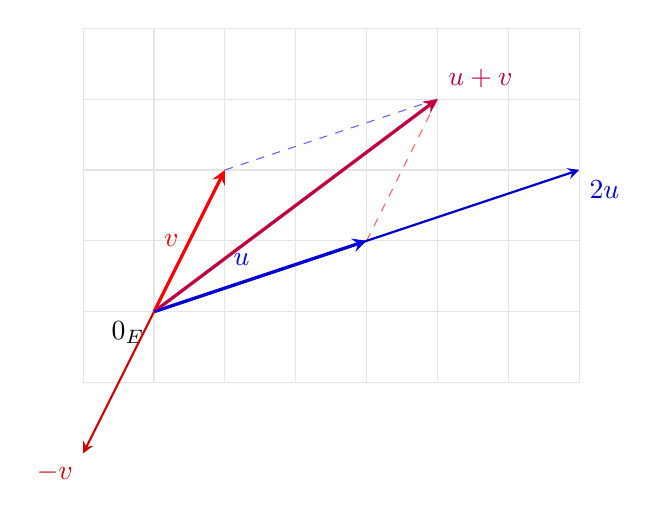
\begin{tikzpicture}[scale=0.9, >=stealth]
    % Grille
    \draw[thin, gray!20] (-1,-1) grid (6,4);
    
    % Origine
    \coordinate (O) at (0,0);
    \node[below left] at (O) {$0_E$};
    
    % Vecteur u
    \draw[->, very thick, blue] (O) -- (3,1) node[midway, above left] {$u$};
    
    % Vecteur v
    \draw[->, very thick, red] (O) -- (1,2) node[midway, left] {$v$};
    
    % Addition u + v (Parallélogramme)
    \draw[dashed, thin, red!60] (3,1) -- (4,3);
    \draw[dashed, thin, blue!60] (1,2) -- (4,3);
    \draw[->, very thick, purple] (O) -- (4,3) node[above right] {$u + v$};
    
    % Scalaire 2u
    \draw[->, thick, blue!80!black] (O) -- (6,2) node[below right] {$2u$};
    
    % Scalaire -v
    \draw[->, thick, red!80!black] (O) -- (-1,-2) node[below left] {$-v$};
\end{tikzpicture}
\end{center}

\paragraph{2. Combinaison linéaire}
Une \textbf{combinaison linéaire} $\lambda_1 v_1 + \lambda_2 v_2$ consiste simplement à parcourir une certaine distance dans la direction de $v_1$ (ajustée par $\lambda_1$), puis à repartir dans la direction de $v_2$ (ajustée par $\lambda_2$).

\begin{center}
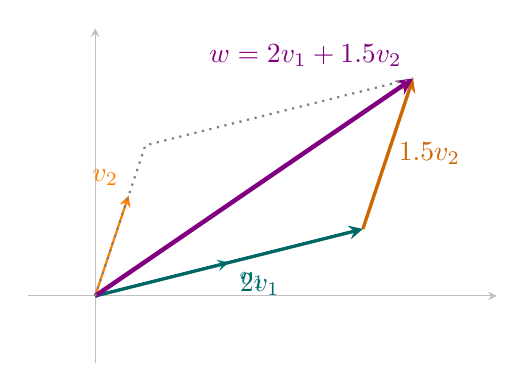
\begin{tikzpicture}[scale=0.85, >=stealth]
    % Axes discrets
    \draw[->, gray!50] (-1,0) -- (6,0);
    \draw[->, gray!50] (0,-1) -- (0,4);
    
    % Origine
    \coordinate (O) at (0,0);
    
    % Vecteurs de base v1 et v2
    \coordinate (V1) at (2,0.5);
    \coordinate (V2) at (0.5,1.5);
    
    \draw[->, thick, teal] (O) -- (V1) node[below right] {$v_1$};
    \draw[->, thick, orange] (O) -- (V2) node[above left] {$v_2$};
    
    % Deplacement 2*v1
    \coordinate (2V1) at (4,1);
    \draw[->, very thick, teal!80!black] (O) -- (2V1) node[midway, below right] {$2 v_1$};
    
    % Deplacement 1.5*v2
    \coordinate (CL) at (4.75, 3.25);
    \draw[->, very thick, orange!80!black] (2V1) -- (CL) node[midway, right] {$1.5 v_2$};
    
    % Résultat
    \draw[->, ultra thick, violet] (O) -- (CL) node[above left] {$w = 2 v_1 + 1.5 v_2$};
    
    % Pointille d'aide
    \draw[dotted, thick, gray] (O) -- (0.75, 2.25) -- (CL);
\end{tikzpicture}
\end{center}

\remark{En jouant sur les coefficients $(\lambda_1, \lambda_2) \in \mathbb{R}^2$, les combinaisons linéaires $\lambda_1 v_1 + \lambda_2 v_2$ de deux vecteurs non alignés permettent d'atteindre \textbf{n'importe quel point} du plan. C'est l'idée fondamentale derrière la notion de \textit{famille génératrice} et de \textit{dimension} que l'on abordera plus tard.}

\remark{On retombe sur nos pattes : on en connaît déjà beaucoup sur les espaces vectoriels, même si on ne le savait pas ! Par exemple, $\mathbb{R}^2$ (et plus généralement $\mathbb{R}^n$) est un espace vectoriel pour les lois usuelles, et on a déjà utilisé des combinaisons linéaires dans le plan.}

\subsection{Sous-espaces vectoriels}

\definition{
    Soit $E$ un $\mathbb{K}$-espace vectoriel. Soit $F \subset E$.\\
    On dit que $F$ est un \textbf{sous-espace vectoriel} \textit{(abrégé "sev")} de $E$ si :
    \begin{itemize}
        \item $F \neq \emptyset$
        \item $\forall u,v \in F, \lambda,\mu \in \mathbb{K}, \lambda u + \mu v \in F$
    \end{itemize}
}

\theorem{Proposition}{Caractérisation des sous-espaces vectoriels}{false}{
    Tout sous-espace vectoriel est un espace vectoriel pour les lois induites par $E$.
}

\noindent{\textbf{Preuve:}\\
Montrons $(F, +)$ est un sous-groupe de $(E, +)$ :\\
\begin{itemize}
    \item $F \neq \emptyset$ donc $\exists u \in F$.
    \item $\lambda = \mu = 1 \implies u + v \in F, \forall u,v \in F$ donc $F$ est stable par $+$
    \item $u + (-1)u = u(1 + (-1)) = 0_E \in F$. On a donc $-u \in F, \forall u \in F$.
\end{itemize}
Donc on a bien un sous-groupe.\\
Les autres propriétés sont vérifiables et immédiates, on a bien un espace vectoriel
}

\example{
    Soit $E$ un $\mathbb{K}$-ev.\\
    \begin{itemize}
        \item $\{0_E\}$ et $E$ sont des sous-ev de $E$.
        \item $\{(x,y) \mid ax+by=0\} \subset \mathbb{R}^2$ est un sous-ev de $\mathbb{R}^2$. En effet, soient $(x,y), (x',y') \in \{(x,y) \mid ax+by=0\}$ et $\lambda, \mu \in \mathbb{R}$.\\
        Alors : $\lambda(x,y) + \mu(x',y') = (\lambda x + \mu x', \lambda y + \mu y')$.\\
        On a $\lambda x + \mu x' = 0$ et $\lambda y + \mu y' = 0$, donc $\lambda(x,y) + \mu(x',y') \in \{(x,y) \mid ax+by=0\}$.
    \end{itemize}
}

\training{Montrer que $\{(x,y,z) \in \mathbb{R}^3 \mid x+y+z=0\}$ est un sous-espace vectoriel de $\mathbb{R}^3$. Quelle est sa nature géométrique ?}
\noindent \carreaux{10}

\method{Montrer qu'un ensemble est un espace vectoriel}{
    Pour montrer que $F \subset E$ est un sous-espace vectoriel, il suffit de vérifier que $F \neq \emptyset$ et que $F$ est stable par combinaison linéaire (\textit{ie.} $\forall u,v \in F, \forall \lambda, \mu \in \mathbb{K}, \lambda u + \mu v \in F$).
}


\theorem{Proposition}{Intersection de sous-espaces vectoriels}{false}{
    Soit $E$ un $\mathbb{K}$-espace vectoriel. Soit $(F_i)_{i \in I}$ une famille de sous-espaces vectoriels de $E$.\\
    Alors $\bigcap_{i \in I} F_i$ est un sous-espace vectoriel de $E$.
}

\noindent{\textbf{Preuve:}\\
Montrons que $\bigcap_{i \in I} F_i$ est stable par combinaison linéaire.\\
Soient $x,y \in \bigcap_{i \in I} F_i$ et $\lambda, \mu \in \mathbb{K}$.\\
On a $x,y \in F_i$ pour tout $i \in I$, donc $\lambda x + \mu y \in F_i$ pour tout $i \in I$.\\
Donc $\lambda x + \mu y \in \bigcap_{i \in I} F_i$. $\Box$}

\attention{Cette proposition est \textbf{FAUSSE} pour l'union de sous-espaces vectoriels.}

\theorem{Proposition}{Sous-ev engendré}{false}{
    Soit $E$ un $\mathbb{K}$-espace vectoriel. Soit $X \subset E$.\\
    Alors il existe un plus petit sous-espace vectoriel de $E$ contenant $X$, noté $\text{Vect}(X)$ et appelé le \textbf{ sous-espace vectoriel engendré} par $X$. On a : $$\text{Vect}(X) = \{\sum_{x\in X} \lambda_x x \mid (\lambda_x)_{x\in X}, \lambda_x \in \mathbb{K}\} = \bigcap_{\substack{F \text{ sous-espace vectoriel de } E \\ X \subset F}} F$$\\\\
    Intuitivement, c'est l'ensemble des combinaisons linéaires d'éléments de $X$, \textit{ie.} l'ensemble des vecteurs que l'on peut obtenir en combinant les vecteurs de $X$ avec des scalaires de $\mathbb{K}$.
}

\noindent{\textbf{Preuve:}\\
Montrons que $Vect(X)$ est un sev de E.\\
Soient $u,v \in Vect(X)$ et $\lambda, \mu \in \mathbb{K}$.\\
On a $u = \sum_{x \in X} \lambda_x x$ et $v = \sum_{x \in X} \mu_x x$ avec $(\lambda_x)_{x \in X}$ et $(\mu_x)_{x \in X}$ presque nulles.\\
Donc $\lambda u + \mu v = \sum_{x \in X} (\lambda \lambda_x + \mu \mu_x) x$ est une combinaison linéaire d'éléments de $X$ avec des coefficients presque nuls.\\
Donc $\lambda u + \mu v \in Vect(X)$. C'est bien un sev.

On a $X \subset \{CL de X\}$ car $x = 1 \cdot x + 0 \cdot y, \forall x \in X, y \in E$.\\
Donc $Vect(X) \subset \{CL de X\}$.\\
Réciproquement, $Vect(X)$ est stable par combinaison linéaire et contient $X$, donc $\{CL de X\} \subset Vect(X)$. Donc $Vect(X) = \{CL de X\}$. $\Box$.}

\remark{Il faut s'arrêter sur cette notion et bien la comprendre. C'est un concept fondamental de l'algèbre linéaire.}

\example{Considérons l'espace vectoriel $E = \mathbb{F}_2^3$ sur le corps $\mathbb{K} = \mathbb{F}_2 = \{0, 1\}$. Soit la partie $X = \{v_1, v_2\} \subset \mathbb{F}_2^3$ avec :
\[
v_1 = (1, 1, 0) \quad \text{et} \quad v_2 = (0, 1, 1)
\]

\paragraph{1. Dénombrement et calcul explicite de $\text{Vect}(X)$}
Comme $\mathbb{K} = \{0, 1\}$, les seuls scalaires disponibles sont $0$ et $1$. Les combinaisons linéaires $\lambda_1 v_1 + \lambda_2 v_2$ ne donnent que $2^2 = 4$ possibilités :

\begin{itemize}
    \item $0 \cdot v_1 + 0 \cdot v_2 = (0, 0, 0)$
    \item $1 \cdot v_1 + 0 \cdot v_2 = (1, 1, 0)$
    \item $0 \cdot v_1 + 1 \cdot v_2 = (0, 1, 1)$
    \item $1 \cdot v_1 + 1 \cdot v_2 = (1, 1, 0) + (0, 1, 1) = (1, 0, 1)$ \quad \textit{(car $1 + 1 = 0$ dans $\mathbb{F}_2$)}
\end{itemize}

On obtient donc le sous-espace vectoriel :
\[
\text{Vect}(X) = \{(0,0,0),\, (1,1,0),\, (0,1,1),\, (1,0,1)\}
\]

\paragraph{2. Représentation géométrique (Cube unité de $\mathbb{F}_2^3$)}
Dans $\mathbb{F}_2^3$, l'espace vectoriel contient $2^3 = 8$ points qui forment les sommets du cube unité. Le sous-espace $\text{Vect}(X)$ correspond à un sous-groupe (un plan à 4 points) passant par l'origine $(0,0,0)$.

\begin{center}
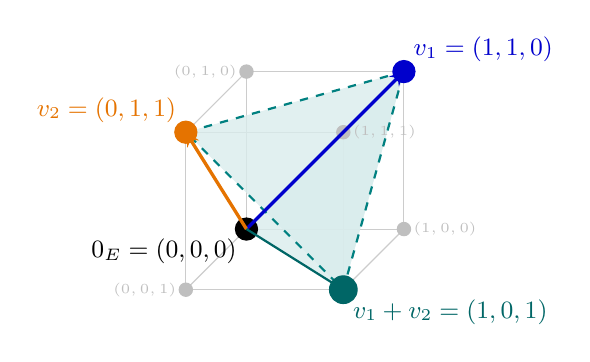
\begin{tikzpicture}[scale=2, >=stealth]
    % Sommets du cube
    \coordinate (000) at (0,0,0);
    \coordinate (100) at (1,0,0);
    \coordinate (010) at (0,1,0);
    \coordinate (001) at (0,0,1);
    \coordinate (110) at (1,1,0);
    \coordinate (011) at (0,1,1);
    \coordinate (101) at (1,0,1);
    \coordinate (111) at (1,1,1);

    % Arêtes du cube global
    \draw[gray!40, thin] (000) -- (100) -- (110) -- (010) -- cycle;
    \draw[gray!40, thin] (001) -- (101) -- (111) -- (011) -- cycle;
    \draw[gray!40, thin] (000) -- (001);
    \draw[gray!40, thin] (100) -- (101);
    \draw[gray!40, thin] (010) -- (011);
    \draw[gray!40, thin] (110) -- (111);

    % Plane / SEV Vect(X) (Zone teinté)
    \fill[teal!15, opacity=0.8] (000) -- (110) -- (101) -- cycle;
    \fill[teal!15, opacity=0.8] (110) -- (011) -- (101) -- cycle;
    \draw[teal, thick, dashed] (110) -- (011) -- (101) -- (110);

    % Points HORS de Vect(X)
    \filldraw[gray!50] (100) circle (1.2pt) node[right, font=\tiny] {$(1,0,0)$};
    \filldraw[gray!50] (010) circle (1.2pt) node[left, font=\tiny] {$(0,1,0)$};
    \filldraw[gray!50] (001) circle (1.2pt) node[left, font=\tiny] {$(0,0,1)$};
    \filldraw[gray!50] (111) circle (1.2pt) node[right, font=\tiny] {$(1,1,1)$};

    % Points DANS Vect(X)
    \filldraw[black] (000) circle (2pt) node[below left, font=\small\bfseries] {$0_E=(0,0,0)$};
    \filldraw[blue!80!black] (110) circle (2pt) node[above right, font=\small\bfseries] {$v_1 = (1,1,0)$};
    \filldraw[orange!90!black] (011) circle (2pt) node[above left, font=\small\bfseries] {$v_2 = (0,1,1)$};
    \filldraw[teal!80!black] (101) circle (2.5pt) node[below right, font=\small\bfseries] {$v_1+v_2 = (1,0,1)$};

    % Vecteurs v1 et v2
    \draw[->, very thick, blue!80!black] (000) -- (110);
    \draw[->, very thick, orange!90!black] (000) -- (011);
    \draw[->, thick, teal!80!black] (000) -- (101);

\end{tikzpicture}
\end{center}}

\remark{Contrairement aux espaces sur $\mathbb{R}$ où un sous-espace engendré par 2 vecteurs non colinéaires contient une infinité de points (un plan continu), sur $\mathbb{F}_2$ il contient un nombre fini d'éléments ($2^{\text{dim}} = 2^2 = 4$ points).}

\theorem{Proposition}{Somme de sous-espaces vectoriels}{false}{
    Soit $E$ un $\mathbb{K}$-espace vectoriel. Soient $F$ et $G$ deux sous-espaces vectoriels de $E$.\\
    Alors $F + G = \{x + y \mid x \in F, y \in G\}$ est un sous-espace vectoriel de $E$.
}

\remark{Cette proposition s'applique à plus que deux espaces vectoriels. En pratique, on préfère noter $F_1 + F_2 + \cdots + F_n$ plutôt que $\sum_{i=1}^n F_i$.}

\theorem{Proposition}{Caractérisation de la somme}{false}{
    Soit $E$ un $\mathbb{K}$-espace vectoriel. Soit $(F_i)_{i \in I}$ une famille de sous-espaces vectoriels de $E$.\\
    Alors $\sum_{i \in I} F_i = \{\sum_{i \in I} x_i \mid x_i \in F_i, \text{ presque tous nuls}\}$.
}

\ndlr{cf. Laurent pour la preuve}

\example{On se place dans $\mathbb{R}^3$. Soit $F_1 = \{(x,0,0) \mid x \in \mathbb{R}\}$ et $F_2 = \{(0,y,0) \mid y \in \mathbb{R}\}$.\\
Alors $F_1 + F_2 = \{(x,y,0) \mid x,y \in \mathbb{R}\}$, c'est le plan d'équation $z=0$.}

\training{Soit $F_1 = \{(x,0,0) \mid x \in \mathbb{R}\}$ et $F_2 = \{(0,y,y) \mid y \in \mathbb{R}\}$. Calculer $F_1 + F_2$.}
\noindent \carreaux{5}

\definition{
    Soient $(F_1, F_2, \ldots, F_n)$ des sous-espaces vectoriels de $E$. On dit que $F_1 + F_2 + \cdots + F_n$ est une \textbf{somme directe} et on note $F_1 \oplus F_2 \oplus \cdots \oplus F_n$ si :
    $$\forall (u_1, u_2, \ldots, u_n) \in F_1 \times F_2 \times \cdots \times F_n, \; u_1 + u_2 + \cdots + u_n = 0_E \implies u_1 = u_2 = \cdots = u_n = 0_E$$
}


\training{Soit $F_1 = \{(x,0,0) \mid x \in \mathbb{R}\}$ et $F_2 = \{(0,y,0) \mid y \in \mathbb{R}\}$. Montrer que $F_1 \oplus F_2$.}
\noindent \carreaux{5}

\vocabulary{Si $F \oplus G = E$, on dit que $F$ et $G$ sont des \textbf{supplémentaires}.}

\theorem{Proposition}{Caractérisation de la somme directe}{false}{
    Soient $F_1, F_2, \ldots, F_n$ des sev de $E$. Les assertions suivantes sont équivalentes :
    \begin{itemize}
        \item $F_1 + F_2 + \cdots + F_n$ est une somme directe.
        \item $\forall (u_1, u_2, \ldots, u_n) \in F_1 \times F_2 \times \cdots \times F_n, u_1 + u_2 + \cdots + u_n = 0_E \implies u_1 = u_2 = \cdots = u_n = 0_E$
        \item $\forall i \in \{1, 2, \ldots, n\}, F_i \cap (F_1 + \cdots + F_{i-1}) = \{0_E\}$
    \end{itemize}
}

\training{Démontrer la proposition précédente.}
\noindent \carreaux{20}

\attention{On a $F_1 \oplus F_2 \Leftrightarrow F_1 \cap F_2 = \{0_E\}$. Mais on pourrait avoir $F_1 \oplus F_2$ et $F_1 \oplus F_3$, et $F_2 \oplus F_3 = \{0_E\}$, et pas forcément $F_1 \oplus F_2 \oplus F_3$.}
\example{Dans $E = \mathbb{R}^2$, considérons trois droites vectorielles distinctes passant par l'origine :
\[
D_1 = \text{Vect}((1,0)), \quad D_2 = \text{Vect}((0,1)), \quad D_3 = \text{Vect}((1,1))
\]

\begin{itemize}
    \item \textbf{Elles engendrent tout l'espace :} $D_1 + D_2 + D_3 = \mathbb{R}^2$.
    \item \textbf{La somme n'est pas directe :} Il existe une combinaison non triviale de vecteurs $u_1 \in D_1$, $u_2 \in D_2$, $u_3 \in D_3$ qui donne le vecteur nul.
\end{itemize}

Par exemple, en prenant $u_1 = (1,0)$, $u_2 = (0,1)$ et $u_3 = (-1,-1)$ :
\[
\underbrace{(1,0)}_{\in D_1} + \underbrace{(0,1)}_{\in D_2} + \underbrace{(-1,-1)}_{\in D_3} = (0,0) = 0_E
\]
Comme ces vecteurs sont non nuls, la somme $D_1 + D_2 + D_3$ \textbf{n'est pas directe}.}

\begin{center}
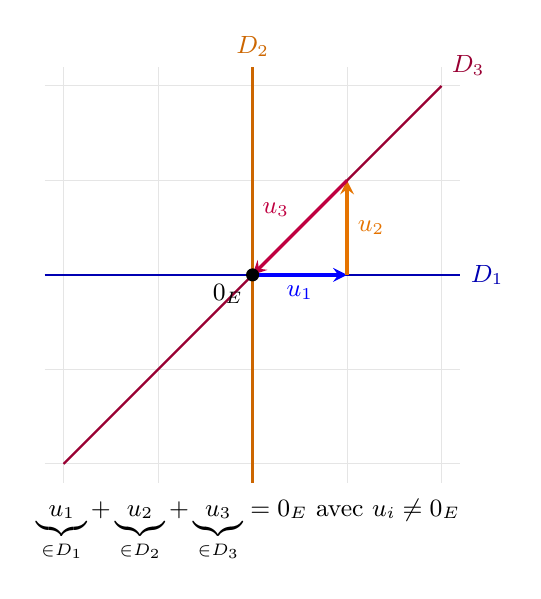
\begin{tikzpicture}[scale=1.2, >=stealth]
    % Grille fine
    \draw[thin, gray!20] (-2.2,-2.2) grid (2.2,2.2);

    % Droites vectorielles
    \draw[thick, blue!70!black] (-2.2,0) -- (2.2,0) node[right, font=\small] {$D_1$};
    \draw[thick, orange!80!black] (0,-2.2) -- (0,2.2) node[above, font=\small] {$D_2$};
    \draw[thick, purple!80!black] (-2,-2) -- (2,2) node[above right, font=\small] {$D_3$};

    % Vecteurs de la décomposition u1 + u2 + u3 = 0
    \draw[->, very thick, blue] (0,0) -- (1,0) node[midway, below, font=\small] {$u_1$};
    \draw[->, very thick, orange!90!black] (1,0) -- (1,1) node[midway, right, font=\small] {$u_2$};
    \draw[->, very thick, purple] (1,1) -- (0,0) node[midway, above left, font=\small] {$u_3$};

    % Origine
    \filldraw[black] (0,0) circle (1.8pt) node[below left, font=\small] {$0_E$};

    % Légende sous le graphique
    \node[align=center, font=\small] at (0,-2.7) {
        $\underbrace{u_1}_{\in D_1} + \underbrace{u_2}_{\in D_2} + \underbrace{u_3}_{\in D_3} = 0_E$ avec $u_i \neq 0_E$
    };
\end{tikzpicture}
\end{center}

\remark{Deux à deux, ces droites sont en somme directe (car $D_i \cap D_j = \{0_E\}$ si $i \neq j$). Cependant, la famille des trois droites n'est pas en somme directe globale. C'est l'un des pièges classiques du cours !}

\attention{Le supplémentaire d'un sous-espace vectoriel n'est pas unique. Par exemple, dans $\mathbb{R}^2$, le sous-espace $D_1 = \text{Vect}((1,0))$ a pour supplémentaire $D_2 = \text{Vect}((0,1))$, mais aussi $D_3 = \text{Vect}((1,1))$.}
\subsection{Familles libres et génératrices}

\definition{
Soit $(x_i)_{i \in I}$ une famille de vecteurs de $E$. On dit que $(x_i)_{i \in I}$ est \textbf{libre} si :

$$\sum_{i \in I} \lambda_i x_i = 0_E \implies \forall i \in I, \lambda_i = 0$$}

\vocabulary{Si $(x_i)_{i \in I}$ n'est pas libre, on dit que c'est une famille \textbf{liée}.}

\example{
    Dans $\mathbb{R}^3$, les vecteurs $(1,0,0)$ et $(0,1,0)$ sont libres.\\
    En effet, si $\lambda_1(1,0,0) + \lambda_2(0,1,0) = (0,0,0)$, on obtient le système :
\[
\begin{cases}
\lambda_1 = 0 \\
\lambda_2 = 0
\end{cases}
\]
À l'inverse, les vecteurs $(1,0,0)$ et $(2,0,0)$ sont liés car $2(1,0,0) - 1(2,0,0) = (0,0,0)$ avec des coefficients non nuls.
}

\training{Soient $u_1 = (1,0,0)$, $u_2 = (0,1,0)$ et $u_3 = (1,1,0)$ dans $\mathbb{R}^3$. La famille $(u_1,u_2,u_3)$ est-elle famille liée ? libre ?}
\noindent \carreaux{10}

\method{Montrer qu'une famille est libre}{
    Deux méthodes, selon ce que vous permet votre cours :
    \begin{itemize}
        \item Montrer que la seule combinaison linéaire qui donne le vecteur nul est la combinaison triviale (tous les coefficients nuls).
        \item Calculer le déterminant de la matrice formée par les vecteurs de la famille (si la famille est finie et que le nombre de vecteurs est égal à la dimension de l'espace). Si le déterminant est non nul, la famille est libre.
    \end{itemize}
}

\example{Explorons le deuxième point. Prenons par exemple la famille de vecteurs $(u_1, u_2, u_3)$ dans $\mathbb{R}^3$ avec :
\[
u_1 = (1,0,0), \quad u_2 = (0,1,0), \quad u_3 = (1,1,0)
\]
On peut former la matrice $A$ dont les colonnes sont les vecteurs $u_1, u_2, u_3$ :
\[
A = \begin{pmatrix}
1 & 0 & 1 \\
0 & 1 & 1 \\
0 & 0 & 0
\end{pmatrix}
\]
Calculons le déterminant de $A$ :
\[\det(A) = 1 \cdot (1 \cdot 0 - 1 \cdot 0) - 0 \cdot (0 \cdot 0 - 1 \cdot 0) + 1 \cdot (0 \cdot 1 - 1 \cdot 0) = 0\]
Le déterminant est nul, donc la famille $(u_1, u_2, u_3)$ est liée.}

\definition{
    Soit $(x_i)_{i \in I}$ une famille de vecteurs de $E$.\\
    On dit que c'est une \textbf{famille génératrice} de $E$ si $Vect(\{x_i \mid i \in I\}) = E$.\\\\
    Alors tout élément de $E$ s'écrit comme une combinaison linéaire des $x_i$.
}

\example{
    Dans $\mathbb{R}^2$, la famille $((1,0),(0,1))$ est génératrice.\\
    En effet, tout vecteur $(x,y) \in \mathbb{R}^2$ s'écrit comme $(x,y) = x(1,0) + y(0,1)$.
}

\training{Soit $u_1 = (1,0,0)$, $u_2 = (0,1,0)$ et $u_3 = (1,1,0)$ dans $\mathbb{R}^3$. La famille $(u_1,u_2,u_3)$ est-elle génératrice de $\mathbb{R}^3$ ?}
\noindent \carreaux{10}

\remark{Il est plus compliqué de montrer qu'une famille est génératrice que de montrer qu'elle est libre. En effet, pour montrer qu'une famille est génératrice, il faut montrer que tout vecteur de l'espace s'écrit comme une combinaison linéaire des vecteurs de la famille. Par chance, on se contentera souvent de montrer qu'une famille est libre, ce qui est plus simple.}

\subsection{Bases}
\definition{
    Soit $(x_i)_{i \in I}$ une famille de vecteurs de $E$ un $\mathbb{K}$-espace vectoriel.\\
    On dit que $(x_i)_{i \in I}$ est une \textbf{base} de $E$ si c'est une famille libre \textbf{et} génératrice de $E$.
}


\theorem{Théorème}{Coordonnées}{false}{
    Soit $(b_i)_{i \in I}$ une base de $E$, et soit $u \in E$.\\
    Alors il existe une unique famille $(\lambda_i)_{i \in I}$ presque nulle telle que $u = \sum_{i \in I} \lambda_i b_i$.
}
\vocabulary{On dit que $\lambda_i$ est la \textbf{i-ème coordonnée} de $u$ dans la base $B$.}
\noindent{\textbf{Preuve:}\\
Montrons l'existence.\\
Comme B est une base, c'est une famille génératrice, donc $u$ s'écrit comme une combinaison linéaire de vecteurs de B.\\
Montrons l'unicité.\\
Supposons qu'il existe $(\lambda_i)_{i \in I}$ et $(\mu_i)_{i \in I}$ presque nulles telles que $u = \sum_{i \in I} \lambda_i b_i = \sum_{i \in I} \mu_i b_i$.\\
On a donc $\sum_{i \in I} (\lambda_i - \mu_i) b_i = 0_E$. Comme B est libre, on a $\forall i \in I, \lambda_i - \mu_i = 0$, donc $\lambda_i = \mu_i$. $\Box$}

\example{E=$\{0\}$, la seule base est la base vide.\\Dans $\mathbb{R}^2$, la famille $((1,0),(0,1))$ est une base : c'est la base canonique.}
\vocabulary{Si $E$ est engendré par une partie finie, on dit que $E$ est de \textbf{dimension finie}.}
\remark{$K^n$ est de dimension finie, $K^X$ avec $X$ infini est de dimension infinie.}

\theorem{Proposition}{}{false}{
    Soit $L \subset E$ avec une partie libre. Soit $u \in E$.\\
    Alors $L \cup \{u\}$ est libre ssi $u \notin Vect(L)$.
}

\noindent{\textbf{Preuve:}\\
Si $u \in Vect(L)$, alors $u = \sum_{v \in L} \lambda_v v$ avec $(\lambda_v)_{v \in L}$ presque nulle.\\
Donc $u - \sum_{v \in L} \lambda_v v = 0
$ avec $1 \neq 0$, donc $L \cup \{u\}$ est liée.\\
Réciproquement, si $L \cup \{u\}$ est liée, alors il existe $(\lambda_v)_{v \in L}$ presque nulle et $\mu \neq 0$ tels que $\sum_{v \in L} \lambda_v v + \mu u = 0_E$.\\
Donc $u = -\frac{1}{\mu} \sum_{v \in L} \lambda_v v \in Vect(L)$. $\Box$}


\theorem{Théorème de la base incomplète}{}{false}{
    Soit $G$ une partie génératrice finie de $E$. Soit $L \subset G$ une partie libre.\\
    Alors il existe une base $B$ de $E$ telle que $L \subset B \subset G$.
}

\remark{Ce théorème est très important. Il permet de compléter une famille libre en une base, ou de réduire une famille génératrice en une base.}

\example{
    Dans $\mathbb{R}^3$, la famille $G = \{(1,0,0), (0,1,0), (0,0,1), (1,1,1)\}$ est génératrice.\\
    La famille $L = \{(1,0,0), (0,1,0)\}$ est libre.\\
    On peut compléter $L$ en une base $B = \{(1,0,0), (0,1,0), (0,0,1)\}$ qui est contenue dans $G$.
}

\training{
    Soit $G = \{(1,0,0), (0,1,0), (0,0,1), (1,1,1)\}$ une partie génératrice de $\mathbb{R}^3$.\\
    Soit $L = \{(1,0,0)\}$ une partie libre.\\
    Compléter $L$ en une base $B$ de $\mathbb{R}^3$ telle que $L \subset B \subset G$.
}
\noindent \carreaux{10}

\theorem{Corollaire}{Existence de base}{false}{
    Si $E$ est un $K$-ev de dimension finie, alors $E$ admet une base.
}

\noindent{\textbf{Preuve:}\\
On applique le théorème de la base incomplète avec $L = \emptyset$. $\Box$}

\theorem{Corollaire}{Caractérisation des bases}{false}{
    Si $L$ est une partie libre à $p$ éléments de $E$ et $G$ une partie génératrice finie à $q$ éléments de $E$.\\
    On a $p \leq q$.
}
\ndlr{cf. Laurent pour les preuve}
  


\theorem{Théorème}{Bases finies}{false}{
    Si $E$ est un $K$-ev de dimension finie, alors toutes les bases de $E$ ont le même cardinal.
}
\noindent{\textbf{Preuve:} Si $E$ est de dimension finie $n$ et $(u_1,\ldots,u_n)$ est une famille libre de E, il existe $(u_{p+1}, \ldots, u_n)$ tels que $(u_1, \ldots, u_n)$ est une base de $E$.\\}

\definition{
    Soit $E$ un $\mathbb{K}$-espace vectoriel de dimension finie.\\
    On appelle \textbf{dimension} de $E$ le cardinal d'une base de $E$.\\
    On note $\dim(E)$ la dimension de $E$.
}

\vocabulary{On appelle \textbf{hyperplan} un sev $H$ de $E$ tel que $\dim(H) = \dim(E) - 1$.}
\vocabulary{On appelle \textbf{droite vectorielle} un sev de dimension 1.}

\method{Montrer qu'une famille de vecteurs est une base d'un espace vectoriel de dimension finie}{
    Il suffit de montrer que la famille est libre et qu'elle contient $\dim(E)$ éléments.
}

\remark{Et c'est beaucoup simple que de montrer qu'une famille est génératrice !}

\theorem{Proposition}{}{false}{
Soit $E$ un $K$-ev. Supposons $E$ de dimension finie.\\
Soit $F$ un sev de $E$. Alors $F$ est de dimension finie et $\dim(F) \leq \dim(E)$.\\\\
Si de plus $\dim(F) = \dim(E)$, alors $F = E$.
}
\ndlr{cf. Laurent pour la preuve}

\section{Applications linéaires}

\definition{
    Soient $E$ et $F$ des $K$-ev.\\
    Soit une application \functionSets{f}{E \rightarrow F}.\\
    On dit que $f$ est une \textbf{application linéaire} si $\forall x,y \in E, \forall \lambda, \mu \in K, f(\lambda x + \mu y) = \lambda f(x) + \mu f(y)$.\\\\
    On note $\mathcal{L}(E,F)$ l'ensemble des applications linéaires de $E$ dans $F$.
}

\vocabulary{On appelle aussi les applications linéaires des \textbf{morphismes} d'espaces vectoriels.}
\remark{$f$ est un morphisme de groupes de $(E,+)$ dans $(F,+)$.}

\vocabulary{On dit que $f$ est un \textbf{endomorphisme} si $E=F$.\\
On dit que $f$ est un \textbf{isomorphisme} si $f$ est bijective.\\
On dit que $f$ est un \textbf{automorphisme} si $f$ est un endomorphisme et un isomorphisme.}

\vocabulary{Si $F=K$, on dit que $f$ est une \textbf{forme linéaire}.}

\example{
    \begin{enumerate}
        \item Soit $\alpha \in K$. L'application \function{\varphi_\alpha}{E \rightarrow E}{x \mapsto \alpha x} est linéaire. C'est l'\textbf{homotétie} de rapport $\alpha$.
        \item Soit $B$ une base de $E$.\\
        L'application \function{\varphi_B}{E \rightarrow}{x \mapsto \text{ième coordonnée de } x \text{ dans la base } B} est linéaire. C'est \textbf{l'application coordonnées} dans la base $B$.
    \end{enumerate}
}

\theorem{Proposition}{}{false}{
    Soit $f \in \mathcal{L}(E,F)$. Soit $B$ une base de $E$.\\
    Alors $f$ est déterminée par ses valeurs sur $B$. \textit{(i.e. si $g \in \mathcal{L}(E,F)$ vérifie $f(e_i) = g(e_i), \forall i$, alors $f=g$)}
}

\remark{
    \begin{itemize}
        \item $B$ génératrice suffit.
        \item Si $E$ est de dimension finie, $f$ est déterminée par un nombre fini de valeurs.
    \end{itemize}
}

\ndlr{cf. Laurent pour la preuve}

\theorem{Proposition}{}{false}{
    $\mathcal{L}(E,F)$ est un $K$-ev.
}

\ndlr{cf. Laurent pour la preuve}


\theorem{Proposition}{Composition d'applications linéaires}{false}{
    Soient $E,F,G$ des $K$-ev. Soient $f \in \mathcal{L}(E,F)$ et $g \in \mathcal{L}(F,G)$.\\
    Alors $g \circ f \in \mathcal{L}(E,G)$.
}

\ndlr{cf. Laurent pour la preuve}


\theorem{Proposition}{}{false}{
    Si on fixe $f \in \mathcal{L}(E,F)$ (respectivement $g \in \mathcal{L}(F,G)$), l'application \function{\varphi_f}{\mathcal{L}(F,G) \rightarrow \mathcal{L}(E,G)}{g \mapsto g \circ f} (resp. \function{\psi_g}{\mathcal{L}(E,F) \rightarrow \mathcal{L}(E,G)}{f \mapsto g \circ f}) est linéaire.
}

\ndlr{cf. Laurent pour la preuve}

\theorem{Proposition}{}{false}{
    Soit $f \in \mathcal{L}(E,F)$ bijective.\\
    Alors $f^{-1} \in \mathcal{L}(F,E)$ et est un isomorphisme.
}

\ndlr{cf. Laurent pour la preuve}


\definition{
    Si $E=F$. Soit $f \in \mathcal{L}(E)$. On définit $f^0 = id_E$ et pour $n \in \mathbb{N}^*, f^n = f \circ f^{n-1}$.\\
    Si $f$ est un automorphisme, on définit pour $n \in \mathbb{N}, f^{-n} = (f^{-1})^n$.
}

\definition{On note $GL(E) = \{f \in \mathcal{L}(E) \mid f \text{ est bijective}\}$ est le groupe linéaire de $E$.}

\theorem{Proposition}{}{false}{
    $GL(E)$ est un groupe pour la composition. 
}

\remark{Si $K$ est un corps fini, i.e. $K = \mathbb{Z}/p\mathbb{Z}$, $p$ premier, et si $E$ est de dimension finie $n$, alors $GL(E)$ est fini.}

\subsection{Noyau et image d'une application linéaire}

\ndlr{Un grand merci à Laurent qui a pris en note cette partie du cours. J'ai omis les démonstrations, voir le cours de l'année précédente pour les détails.}

\definition{
    Soit $f \in \mathcal{L}(E,F)$. On définit le \textbf{noyau} de $f$ par : $\ker(f) = f^{-1}(0_E) = \{x \in E \mid f(x) = 0_F\}$.\\
    On définit l'\textbf{image} de $f$ par : $\text{Im}(f) = f(E) = \{f(x) \mid x \in E\}$.
}
\vocabulary{On appelle \textbf{rang} de $f$ la dimension de $\text{Im}(f)$, notée $\text{rg}(f)$.}
\theorem{Proposition}{}{true}{
    Soit $f \in \mathcal{L}(E,F)$. Alors $\ker(f)$ est un sev de $E$ et $\text{Im}(f)$ est un sev de $F$.
}
\theorem{Proposition}{Injectivité}{true}{
    Soit $f \in \mathcal{L}(E,F)$. Alors $f$ est injective si et seulement si $\ker(f) = \{0_E\}$.
}
\theorem{Proposition}{Surjectivité}{true}{
    Soit $f \in \mathcal{L}(E,F)$. Alors $f$ est surjective si et seulement si $\text{Im}(f) = F$.
}
\theorem{Théorème du rang}{}{true}{
    Supposons $E$ de dimension finie. Alors $\ker(f)$ et $\text{Im}(f)$ sont de dimension finie et on a : \[\dim(E) = \dim(\ker(f)) + \dim(\text{Im}(f))\].
}

\remark{Le rang d'une famille de vecteurs $(x_1,\ldots,x_k)$ est la dimension de $Vect(\{x_i\})$.}

\theorem{Corollaire}{}{true} {
    On suppose $E$ de dimension finie. 
    \begin{enumerate}
        \item Si $f$ est injective, alors $\dim(F) \geq \dim(E)$.
        \item Si $f$ est surjective, alors $\dim(F) \leq \dim(E)$.
        \item Si $f$ est bijective, alors $\dim(F) = \dim(E)$.
        \item Si $F$ est de dimension finie, et $\dim(E) = \dim(F)$, alors les assertions suivantes sont équivalentes :
        \begin{itemize}
            \item $f$ est bijective
            \item $f$ est injective
            \item $f$ est surjective
        \end{itemize}
    \end{enumerate}
}

\subsection{Espaces vectoriels produits}

\theorem{Proposition}{Construction}{true}{
    Soient $E,F$ des $K$-ev. Alors $E \times F$ est un groupe produit pour $+$.
    On munit $E \times F$ de la multiplication externe donnée par \function{\cdot}{K \times (E \times F) \rightarrow E \times F}{(\lambda, (x,y)) \mapsto (\lambda x, \lambda y)}.\\
    Alors $E \times F$ est un $K$-ev, appelé \textbf{espace-vectoriel produit} de $E$ et $F$.
}

\remark{Si $E_1 \ldots E_n$ sont des $K$-ev, on définit de même le $K$-ev produit $E_1 \times E_2 \times \cdots \times E_n$. En particulier, $E^n = E \times E \times \cdots \times E$.}

\theorem{Proposition}{Base et dimension de l'espace-vectoriel produit}{true}{
    Soient $(b_i)_{i \in I}$ une base de $E$ et $(c_j)_{j \in J}$ une base de $F$, et $I \cap J = \emptyset$.\\
    Alors la famille $(d_k)_{k \in I \cup J}$ définie par $d_i = (b_i, 0_F)$ si $i \in I$ et $d_i = (0_E, c_i)$ si $i \in J$ est une base de $E \times F$.\\
    En particulier, si $E$ et $F$ sont de dimension finies, $E \times F$ est de dimension finie et $\dim(E \times F) = \dim(E) + \dim(F)$.
}

\theorem{Propriété}{}{true}{
    On sait que $K$ est un $K$-ev de dimension 1, de base $\{1\}$.\\
    Donc pour $n \geq 1$, $K^n$ est de dimension $n$ et de base canonique $\{e_1, e_2, \ldots, e_n\}$ où $e_i$ est le vecteur dont la i-ème coordonnée vaut 1 et les autres 0.
}
\vocabulary{Une telle base est appelée la \textbf{base canonique} de $K^n$.}

\theorem{Proposition}{Espace vectoriel de dimension égale}{true}{
    Soit $E$ un $K$-ev de dimension finie $n$ et base $B = (b_i)_{1 \leq i \leq n}$.\\
    Il existe un isomorphisme de $E$ sur $K^n$ qui à $\sum_{i=1}^n \lambda_i b_i \mapsto \sum_{i=1}^n \lambda_i e_i$.\\
}

\theorem{Théorème}{Isomorphisme sur $K^n$}{true}{
    Tout espace vectoriel de dimension finie $n$ est isomorphe à $K^n$.
}
\remark{Cet isomorphisme dépend du choix d'une base et n'est pas unique.}

\theorem{Théorème}{Généralisation de l'isomorphime de deux espaces vectoriels}{true}{
    Soient $E$ et $F$ deux $K$-ev de dimension finie.\\
    Alors $E$ et $F$ sont isomorphes si et seulement si $\dim(E) = \dim(F)$.
}

\subsection{Sommes et supplémentaires}

\theorem{Proposition}{Formule de Grassman}{true}{
    Soit $E$ un $K$-ev de dimension finie. Soient $F$ et $G$ deux sev de $E$.\\
    Alors $F + G$ est de dimension finie et on a : \[\dim(F + G) = \dim(F) + \dim(G) - \dim(F \cap G)\].
}

\theorem{Corollaire}{}{true}{
    Si $F$ et $G$ sont en somme directe, alors on a $F \oplus G$ est isomorphe à $F \times G$.
}

\theorem{Proposition}{Existence de supplémentaires}{true}{
    Soit $E$ un $K$-ev de dimension finie. Soit $F$ un sev de $E$.\\
    Alors il existe un sev (non unique) $G$ de $E$ tel que $F \oplus G = E$.
}

\theorem{Propriété}{}{true}{
    Supposons que $F \oplus G = E$.\\
    Tout $x\in E$ s'écrit de manière unique $x = y + z$ avec $y \in F$ et $z \in G$.
}
\definition{
    On appelle \textbf{projection sur $F$ parallèlement à $G$} l'application \function{\pi_{F,G}}{E \rightarrow E}{x = y + z \mapsto y} où $y \in F$ et $z \in G$.\\
}

\theorem{Proposition}{}{true}{
    \begin{enumerate}
        \item On a $p(x) = x$ si $x \in F$.
        \item On a $p(x) = 0_E$ si $x \in G$.
        \item On a $p(x) = 0$ so $F = \{0_E\}$.
        \item On a $p(x) = id$ si $F = E$.
        \item On a $p \circ p = p$ (on dit que $p$ est idempotente).
        \item L'endomorphisme $id_E - p$ est la projection sur $G$ parallèlement à $F$.
    \end{enumerate}
}

\theorem{Proposition}{Projection et noyau}{true}{
    Soit $p \in \mathcal{L}(E)$ tel que $p \circ p = p$.\\
    Alors on a $\ker(p) \oplus \text{Im}(p) = E$ et $p$ est la projection sur $\text{Im}(p)$ parallèlement à $\ker(p)$.
}

\definition{
    Soit $E$ un $K$-ev de dimension finie. Soient $F$ et $G$ deux sev de $E$.\\
    On appelle \textbf{symétrie par rapport à $F$ parallèlement à $G$} l'application \function{s_{F,G}}{E \rightarrow E}{x = y + z \mapsto y - z} où $y \in F$ et $z \in G$.\\
}

\theorem{Proposition}{}{true}{
    On a $s = 2p - id_E$ où $p$ est la projection sur $F$ parallèlement à $G$.\\
}

\theorem{Proposition}{}{true}{
    On a $s^2 = id_E$.
}

\theorem{Proposition}{}{true}{
    Soit $s \in \mathcal{L}(E)$ tel que $s^2 = id_E$.\\
    Alors on a $E = \ker(s - id_E) \oplus \ker(s + id_E)$ et $s$ est la symétrie par rapport à $\ker(s - id_E)$ parallèlement à $\ker(s + id_E)$.
}

\section{Matrices représentatives}
\section{Réduction des endomorphismes}

\newpage
\tableofcontents
\end{document}